%%%%%%%%%%%%%%%%%%%%%%%%%%%%%%%%%%%%%%%%%%%%%%%%%%%%%%%%%%
%
% Vzor pro sazbu kvalifikační práce
%
% Západočeská univerzita v Plzni
% Fakulta aplikovaných věd
% Katedra informatiky a výpočetní techniky
%
% Petr Lobaz, lobaz@kiv.zcu.cz, 2016/03/14
%
%%%%%%%%%%%%%%%%%%%%%%%%%%%%%%%%%%%%%%%%%%%%%%%%%%%%%%%%%%

% Možné jazyky práce: czech, english
% Možné typy práce: BP (bakalářská), DP (diplomová)
\documentclass[czech,DP]{thesiskiv}

% Definujte údaje pro vstupní strany
%
% Jméno a příjmení; kvůli textu prohlášení určete, 
% zda jde o mužské, nebo ženské jméno.
\author{Zdeněk Valeš}
\declarationmale

%alternativa: 
%\declarationfemale

% Název práce
\title{Určování nahraditelnosti a\\kompatibility webových služeba}

% 
% Texty abstraktů (anglicky, česky)
%
\abstracttexten{The text of the abstract (in English). It contains the English translation of the thesis title and a short description of the thesis.}

\abstracttextcz{Text abstraktu (česky). Obsahuje krátkou anotaci (cca 10 řádek) v češtině. Budete ji potřebovat i při vyplňování údajů o bakalářské práci ve STAGu. Český i anglický abstrakt by měly být na stejné stránce a měly by si obsahem co možná nejvíce odpovídat (samozřejmě není možný doslovný překlad!).
}

% Na titulní stranu a do textu prohlášení se automaticky vkládá 
% aktuální rok, resp. datum. Můžete je změnit:
%\titlepageyear{2016}
%\declarationdate{1. března 2016}

% Ve zvláštních případech je možné ovlivnit i ostatní texty:
%
%\university{Západočeská univerzita v Plzni}
%\faculty{Fakulta aplikovaných věd}
%\department{Katedra informatiky a výpočetní techniky}
%\subject{Bakalářská práce}
%\titlepagetown{Plzeň}
%\declarationtown{Plzni}

%%%%%%%%%%%%%%%%%%%%%%%%%%%%%%%%%%%%%%%%%%%%%%%%%%%%%%%%%%
%
% DODATEČNÉ BALÍČKY PRO SAZBU
% Jejich užívání či neužívání záleží na libovůli autora 
% práce
%
%%%%%%%%%%%%%%%%%%%%%%%%%%%%%%%%%%%%%%%%%%%%%%%%%%%%%%%%%%

% Zařadit literaturu do obsahu
\usepackage[nottoc,notlot,notlof]{tocbibind}

% Umožňuje vkládání obrázků
\usepackage[pdftex]{graphicx}
\graphicspath{{./img/}}

% Odkazy v PDF jsou aktivní; navíc se automaticky vkládá
% balíček 'url', který umožňuje např. dělení slov
% uvnitř URL
\usepackage[pdftex]{hyperref}
\hypersetup{colorlinks=true,
  unicode=true,
  linkcolor=black,
  citecolor=black,
  urlcolor=black,
  bookmarksopen=true}

% Při používání citačního stylu csplainnatkiv
% (odvozen z csplainnat, http://repo.or.cz/w/csplainnat.git)
% lze snadno modifikovat vzhled citací v textu
\usepackage[numbers,sort&compress]{natbib}


% na seznam zktratek
\usepackage{longtable}
\newcommand\nomenclature[2]{#1 & #2 \\}

%%%%%%%%%%%%%%%%%%%%%%%%%%%%%%%%%%%%%%%%%%%%%%%%%%%%%%%%%%
%
% VLASTNÍ TEXT PRÁCE
%
%%%%%%%%%%%%%%%%%%%%%%%%%%%%%%%%%%%%%%%%%%%%%%%%%%%%%%%%%%
\begin{document}
%
\maketitle
\tableofcontents

\chapter{Úvod}

- k čemu je práce dobrá
- co text práce obahuje
- use casy

\chapter{Principy webových služeb, techniky}
\label{sec:web-services-principles}

V této kapitole jsou definovány webové služby a související pojmy. Jsou zde představeny strojově čitelné způsoby popisu rozhraní služeb a protokoly sloužící ke komunikaci s webovými službami. Tato kapitola také obsahuje popis REST. 

%co je v téhle kapitole:
%
% - co jsou to webové služby
% - k čemu webové služby jsou
% - co je to REST (protože se to přímo dotýká mé práce)
% - co je to API
% - protokoly skrze které se s WS komunikuje
% - strojově čitelné formáty popisu ws

\section{Webové služby}

Pojem 'webová služba' má různé významy pro různé lidi, ale dá se najít několik společných bodů \cite{w3cWsDesignIssues}:
\begin{itemize}
	\item Použití HTML, XML a dalších standardů webové architektury jako stavebních kamenů
	\item Zaměření na podnikové a vnitropodnikové operace
\end{itemize}

% v citovaném článku je spousta zajímavých informací o WS, např "The fact that data is exchanged for business purposes and between different social entities means that accountability is required, rather than just reliable transmission. "
 - pro účely této práce je použita následující definice od W3C \cite{w3cWsArch}:
 "Webová služba je softwarový systém navržený pro podporu mezistrojové komunikace po síti. Webová služba má rozhraní, které je popsáno ve strojově čitelném formátu (konkrétně WSDL). Ostatní systémy interagují s webovými službami předepsaným způsobem za použití zpráv protokolu SOAP, které jsou typicky zprostředkované protokolem HTTP s využitím serializace XML a dalších webových standardů."
 
 % A Web service is a software system designed to support interoperable machine-to-machine interaction over a network. It has an interface described in a machine-processable format (specifically WSDL). Other systems interact with the Web service in a manner prescribed by its description using SOAP messages, typically conveyed using HTTP with an XML serialization in conjunction with other Web-related standards.

- poskytovatel služby = server

- konzument služby = klient (typicky nějaká aplikace)

% zmínit:
% zmínit RPC, SOAP
%- popis použitých technologií: XML, SOAP, WSDL

\section{REST}

%
% - co je REST
% - jak se liší od WS definované v předchozí sekci
% - základní popis elementů použitých v REST

- mohlo by se hodit: https://www.w3.org/TR/2004/NOTE-ws-arch-20040211/\#relwwwrest
- popisuje vztah REST a WWW
- REST: založeno na manipulaci s XML reprezentací webových resources skrze stateless operace

 - popis architektonického stylu REST: https://www.ics.uci.edu/~fielding/pubs/dissertation/rest\_arch\_style.htm
- popis elementů:
- data, konektory, komponenty
- popis view(na modelování)

- RFC na HTTP: https://tools.ietf.org/html/rfc7231\#section-4

- odkaz konkrétně na request methods, mohlo by se hodit, protože ty jsou indexovány, tak alespoň na citaci

\subsection{Technologie použité k realizaci webových služeb}

- zmínit: RPC, SOAP

\begin{figure}
	\centering
	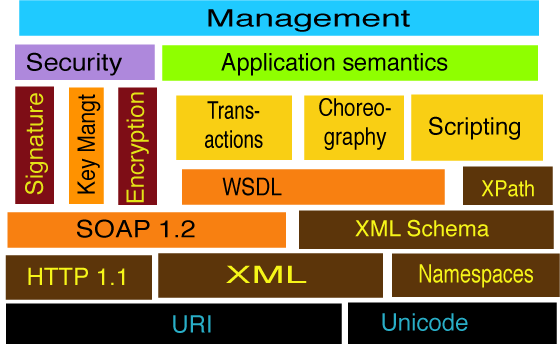
\includegraphics[width=\linewidth]{ws-tech-stack.png}
	\caption{Technologie zahrnuté ve webových službách}
	\label{fig:ws-tech-stack}	
\end{figure}

\section{Protokoly}

- relevantní protokoly: RPC, SOAP, HTTP

- HTTP (na REST a WS obecně)

- protokol aplikační vrstvy SOAP (web service)

- XML pro popis datového modelu

- specifikace SOAP: https://www.w3.org/TR/soap12-part1/\#intro

\section{Formální popis webových služeb}

- existují různé, strojově čitelné, formáty pro popis API

- WSDL 1.1, 2.0, WADL (REST), JSON-WSP

- Swagger, Raml, OpenApi

- v případě REST bohužel není nic formálně nutné (oproti třeba SOAP), takže specifikace API nemusí být kompatibilní, nemusí být úplné, nebo můžou být ad-hoc (např. slovní popis ve Word dokumentu) a tím pádem nemusí existovat univerzální způsob strojového čtení těchto specifikací

- v mé práci se věnuji především formátům WSDL, WADL a JSON-WSP
 
\chapter{Datové typy a porovnávání}

- přednášky z FJP
- jak jazyky řeší datové typy
	- rekurzivní vs. nerekurzivní
- primitivní typy (v xsd)
- built-in typy (v Jave)
- tady budu citovat \cite{abadi1995subytping}
	- subtyping: A <: B <=> A může být použito v kdekoliv kde je očekáváno B
	- kontravariance: F'(A) <: F(B) <=> B <: A

\subsection{Porovnávání datových typů}

 - jak to funguje
 - problémy při porovnání
 - subtyping vs. matching (\cite{abadi1995subytping})


\chapter{Získávání metadat webových služeb v CRCE}

Cílem této práce je vytvořit rozšíření pro úložiště CRCE\footnote{Component Repository supporting Compatibility Evaluation}, které bude schopno vyhodnocovat vzájemnou kompatibilitu indexovaných webových služeb. Tato kapitola představuje samotné úložiště, formát metadat a obecný způsob jejich získání. Na konci kapitoly je popsán princip fungování konkrétních rozšíření, která indexují webové služby (tzv. indexery).

\section{CRCE}

CRCE je komponentové úložiště dlouhodobě vyvíjené a spravované výzkumnou skupinou ReliSA na Katedře Informatiky ZČU, jehož primárním účelem je indexace a následná kontrola vzájemné kompatibility komponent. Úložiště je postaveno na modulární architektuře (viz obrázek \ref{fig:crce-arch}) a je tedy možné přidat rozšíření pro indexaci a zpracování vlastních dat.

\begin{figure}[h]
	\centering
	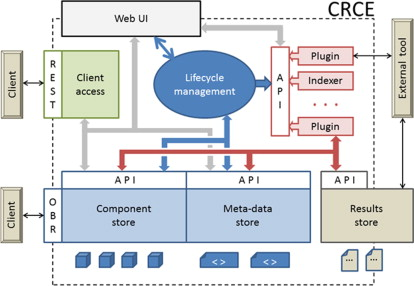
\includegraphics[width=10cm]{crce-arch.jpg}
	\caption{Architektura CRCE}
	\label{fig:crce-arch}
\end{figure} 

\subsection{Metadata komponent}
\label{subsec:crce-metadata}

Data, která vzniknou indexací komponenty a případným dalším zpracováním (např. porovnáním) jsou uložena do souboru metadat a představují klíčový element systému CRCE. Návrh struktury  těchto metadat, který je naznačen na obrázku \ref{fig:crce-resource-uml}, vychází z konceptu OBR\footnote{OSGi bundle repository} jehož základními entitami jsou mimo jiné \textit{Resource}, \textit{requirements} a \textit{capabilities}\cite{brada2015repository}. 

Entita \textit{Resource} reprezentuje komponentu uloženou v CRCE, \textit{requirements} a \textit{capabilities} jsou množiny vlastností, popisující co komponenta ke své správné funkci vyžaduje, respektive co naopak poskytuje. Model také umožňuje přidání key-value atributů k jednotlivým vlastnostem a jejich detailům.
 
 \begin{figure}[h]
 	\centering
 	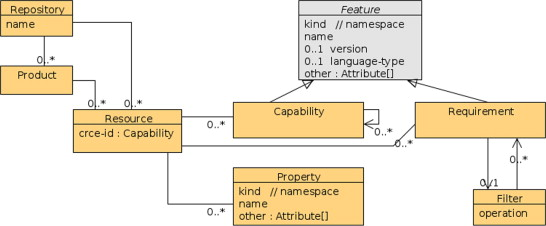
\includegraphics{resource-uml}
 	\caption{Reprezentace metadat v CRCE}
 	\label{fig:crce-resource-uml}
 \end{figure}

V mé práci jsem pracoval především s poskytovanými vlastnostmi (množina \textit{capabilities}) a proto zde popíši hlavně jejich strukturu. Každá konkrétní vlastnost je reprezentována elementem \textit{Capability} a od ostatních je odlišena identifikátorem \textit{namespace}. Detaily konkrétní vlastnosti jsou popsány elementy \textit{Property} a \textit{Attribute}, kde \textit{Property} reprezentuje logický celek několika atributů. Například parametr endpointu REST služby shlukuje atributy popisující jeho jméno, datový typ atp. \textit{Attribute} pak představuje pár klíč-hodnota, který nese konkrétní informace jako např. jméno endpointu, nebo datový typ parametru.

Z obrázku \ref{fig:crce-resource-uml} je vidět rekurzivní povaha elementu \textit{Capability}, čehož je využito ke skládání jednodušších vlastností do složitějších celků. Vznikne tím stromová struktura, která je vhodná k modelování hierarchických dat mezi něž patří například popisy webových služeb. V případě takto komplexních vlastností je ke komponentně (\textit{Resource}) přiřazena pouze jedna, tzv. kořenová, \textit{Capability}, která reprezentuje celou vlastnost.

%Metadata v CRCE mají hierachickou strukturu:
%- Resource + Capability + Properties + Atributy
%- taky Requirements, ale ty v práci nepoužívám
%- Resource reprezentuje indexovanou komponentu
%- jednotlivé featury (indexovaná data) jsou reprezantovány stromem Capabilit
%- k Resource je vždy přiřazena root Capabilita
%- každá Capabilita má namespace, podle kterého lze určit co za konkrétní vlastnost popisuje
%- v případě root Capability by namespace měl být unikátní pro Resource (a resource by tedy neměl mít více root Capabilit s jedním namespace (snad?))
%- detaily fetatury jsou pak uloženy v dětských capabilitách, jejich Properties a Attributes
%- Capability mají Attributy + Properties
%- Properties mají atributy
%- Attributes pak nesou konkrétní hodnoty (Capability a Propeties slouží pouze jako jakési kontejnery)
%- Lze tak modelovat různé vlastnosti indexovaného objektu (viz \cite{brada2015repository}, tam je to dobře popsaný)
%- hierarchická struktura metadat je vhodná pro reprezentaci webových API, která jsou rovněž hierarchická

\subsection{Životní cyklus komponenty v CRCE}

Úložiště bylo primárně navrženo pro ukládání OSGi komponent, nicméně indexovat lze jakýkoliv soubor. Komponenta je v CRCE popsána již zmíněnými metadaty a prochází vlastním životním cyklem naznačeným na obrázku \ref{fig:crce-comp-lc}.

\begin{figure}[h]
	\centering
	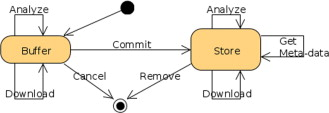
\includegraphics{crce-component-lc.jpg}
	\caption{Životní cyklus komponenty v CRCE}
	\label{fig:crce-comp-lc}
\end{figure} 

Životní cyklus má dvě hlavní fáze, jimiž jsou \textit{Buffer} a \textit{Store}. V obou fázích jsou nad komponentou prováděny operace z nichž \textit{analyze} je nejvíce relevantní mé práci, protože právě během této operace dochází ke sběru metadat (fáze \textit{Buffer}) a dalším výpočtům nad nimi (fáze \textit{Store}). Modul s rozšířením, který je předmětem mé práce bude zařazen mezi výpočty prováděné nad metadaty během \textit{analyze}, kde bude vyhodnocovat vzájemnou kompatibilitu webových služeb. Způsoby sběru těchto metadat, ke kterým dochází ve fázi \textit{Store}, jsou popsány v následující sekci. 

%
%- primárně komponenta = OSGI bundle, ale může být cokoliv (např i pouhý textový soubor)
%
%- nahrání do bufferu
%
%- analýza
%
%- commit do store
%
%- další analýza
%
%- během toho se vytvářejí metadata
%
%- jednotlivé fáze mají callbacky, na které je možné v modulu navěsit vlastní funkcionalitu (\textit{BeforeUploadToBuffer}, \textit{AfterUploadToBuffer}, \textit{BeforeCommit}, ...)

\section{Indexování webových služeb}
\label{sec:api-index}

V této podkapitole je krátce popsán obecný způsob indexace komponent v CRCE. Následně je podrobněji rozebráno indexování webových služeb konkrétními moduly a reprezentace popisu API metadaty v CRCE. Na závěr jsou také uvedeny limity indexování.


\subsection{Obecná indexace komponenty}

Indexace komponenty a související sběr metadat je proveden ve fázi \textit{Buffer} k tomu určenými moduly. Ty jsou vzájemně nezávislé a obecně platí, že každý nich je zaměřen na sběr nějaké logicky ucelené části dat jako například informace o OSGi bundlu, maven koordináty, nebo popis webových služeb. Vlastní data komponenty zůstávají během tohoto procesu nezměněná což v kombinaci s řetězením indexerů zaručuje mimo snadnou rozšiřitelnost také transparentní přístup ke komponentě každému z nich. 

\subsection{Indexace komponenty s webovou službou}

Soubor obsahující implementaci, nebo popis API je v CRCE vnímán jako komponenta a prochází tedy zmíněným životním cyklem včetně výše popsané indexace. Pro popis webových služeb existuje mnoho standardních i nestandardních způsobů, jak již bylo zmíněno v kapitole \ref{sec:web-services-principles}. Z tohoto důvodu je není možné všechny analyzovat jedním indexerem a je nutné zaměřit se pouze na část z nich. 

V současné době tedy existují dva moduly podporující několik popisných formátů a implementací. Konkrétně se jedná o modul pro indexaci webových služeb založených na architektonickém stylu REST\cite{hessova2015rest} a o modul pro indexaci webových služeb s popisem ve formátu WSDL, WADL, nebo Json-WSP \cite{pejrimovsky2015ws}. Oba dva vznikly v rámci diplomových prací a jsou stručně popsány v následujících sekcích.

%- někde by asi bylo fajn ustanovit názvosloví použité v práci:
%\begin{itemize}
%	\item co je API: interface přístupné skrze síť (internet)
%	\item co je web service: service popsaný WSDL, WADL, nebo Json-WSP dokumentem
%	\item co je service: Service element in WSDL
%	\item co je endpoint
%	\item WSDL: port+operation
%	\item endpoint: REST, WADL, JSON-WSP
%\end{itemize}

\begin{figure}[h]
	\centering
	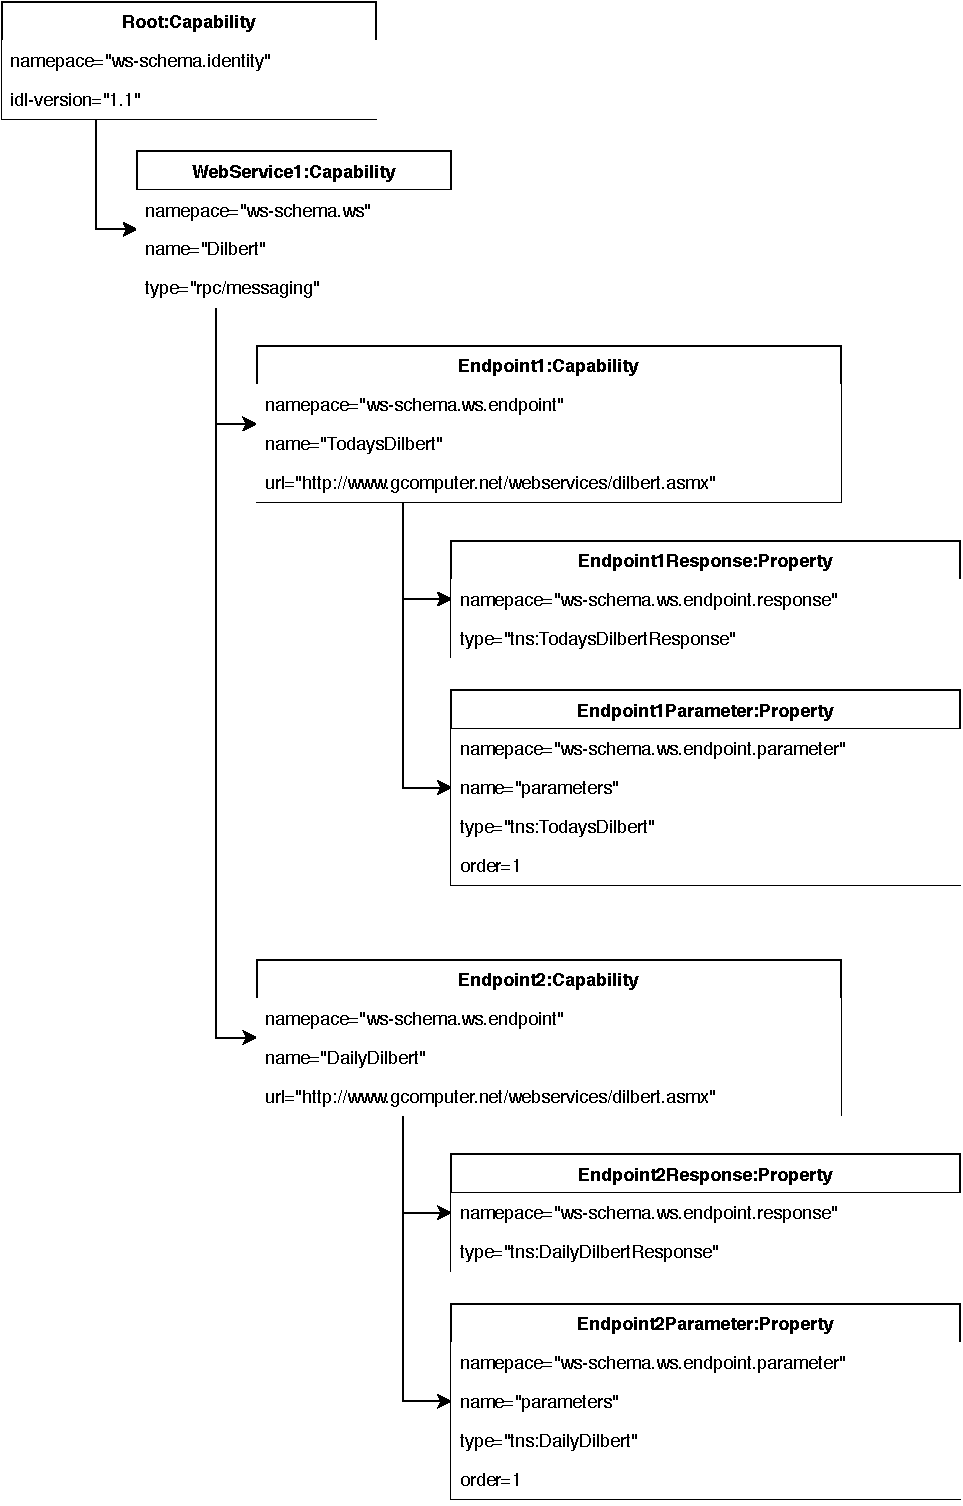
\includegraphics[height=11cm]{indexed-api-example}
	\caption{Příklad indexované SOAP webové služby pro komix Dilbert }
	\label{fig:indexed-api-example}
\end{figure}

\subsection{Struktura metadat popisující webovou službu}

Jak již bylo zmíněno v části \ref{subsec:crce-metadata}, hierarchickou strukturu popisu API lze vhodně vyjádřit metadaty CRCE. Během indexování komponenty reprezentující API jsou shromážděny různé typy popisných vlastností. Jedním z těchto typů je i samotný popis webové služby, který je reprezentován stromem metadat a ke komponentě je přiřazen skrze  kořenovou \textit{Capability}.   

I když jsou různé druhy API indexovány rozdílnými moduly, výsledná metadata mají podobnou strukturu. Příklad metadat API je zobrazen na objektovém diagramu \ref{fig:indexed-api-example}, jedná se o webovou službu, která vrací strip komixu Dilbert pro dnešní den.

Z uvedeného obrázku je vidět, že klíčové elementy API jako web service, nebo endpoint jsou reprezentovány objektem \textit{Capability}. Detaily těchto elementů jsou popsány objekty \textit{Property}. Jedná se zejména o parametry endpointů, těla requestů a response. Objekt \textit{Attribute} pak představuje konkrétní hodnoty, jež jsou na obrázku naznačeny jen jako páry "klíč=hodnota". \textit{Attribute} nemusí být vázaný jen na \textit{Property} a lze jej použít i pro popis \textit{Capability}, jak je tomu např. u objektu \textit{WebService1}.

\subsection{Indexování REST služeb}

Modul pro indexování REST API vznikl v rámci diplomové práce Bc. Gabriely Hessové. Princip sběru dat je založen na binární analýze java archivů (JAR) obsahujících implementaci REST služeb pomocí frameworků splňujících specifikaci JAX-RS a frameworku Spring Web MVC. Modul byl testován na frameworcích Jersey verze 2.26, RESTEasy verze 3.0.16 a  Spring Boot verze 1.5.9 \cite{hessova2015rest}.

Z implementace REST služby modul rekonstruuje kolekci endpointů s jejich parametry, tělem requestu, response a případnými parametry response. Každý endpoint je reprezentován entitou \textit{Capability}, všechny další jeho vlastnosti pak entitami \textit{Property}. Výčet všech indexovaných elementů rozhraní je uveden v tabulce \ref{tab:rest-indexed}.

\begin{table}[h]
	\centering
	\begin{tabular}{|l | c | c |}
		\hline
		Element API & Entita v metadatech & Vstaženo k\\
		\hline
		\hline
		Endpoint & Capability & - \\
		\hline
		Request body & Property & Endpoint \\
		\hline
		Request parameter & Property & Request \\
		\hline
		Response & Property Endpoint & Endpoint \\
		\hline
		Response parameter & Property & Response \\
		\hline
	\end{tabular}
	\caption{Seznam indexovaných elementů REST služby a jejich reprezentací v metadatech}
	\label{tab:rest-indexed}
\end{table}

\subsection{Indexování webových služeb na základě popisu}

Modul pro indexování webových služeb vznikl v rámci práce Bc. Davida Pejřimovského. Oproti předchozímu modulu pro indexaci REST služeb nepracuje tento s její implementací, ale s pouhým popisem. Podporované formáty popisu služeb jsou WSDL (verze 1.1 i 2.0) pro SOAP webové služby, WADL a Json-WSP pro REST služby\cite{pejrimovsky2015ws}.

Struktura dat vytvořených pro REST služby (tedy z popisu WADL, nebo Json-WSP) je podobná struktuře dat vytvořenou předchozím indexerem. Endpoint je tedy reprezentován entitou \textit{Capability}, jeho parametry entitami \textit{Property}. Z popisu Json-WSP je ještě vytvořena reprezentace response pro daný endpoint (entita \textit{Property}). Z popisu WADL se žádné další vlastnosti endpointů nezískávají.

Z WSDL popisu je vytvořena reprezentace služeb, jež jsou popsány xml elementy \verb|<wsdl:service>| a jejich vnořených endpointů. Endpoint je ve WSDL popsán elementem \verb|<wsdl:port>| a má definované operace (elementy \verb|<wsdl:operation>|), nicméně modul tyto nevnořuje a vytváří zjednodušenou reprezentaci. Model endpointu tedy obsahuje metadata získaná z elementů \verb|<wsdl:operation>| a url definovanou v elementu \verb|<wsdl:port>|. Služby i endpointy jsou v metadatech reprezentovány entitami \textit{Capability}. Oproti REST službám, které mají jednu úroveň vnoření \textit{Capability}, zde vznikají úrovně dvě. Výčet elementů API a jejich reprezentace v metadatech je uveden v tabulce \ref{tab:ws-indexed}.

\begin{table}[h]
	\centering
	\begin{tabular}{|l | c | c |}
		\hline
		Element API & Entita v metadatech & Vstaženo k \\
		\hline
		\hline
		Service & Capability & - \\
		\hline
		Endpoint & Capability & Service \\
		\hline
		Endpoint parameter & Property & Endpoint \\
		\hline
		Response & Property & Endpoint \\
		\hline
		Response parameter & Property & Endpoint \\
		\hline
	\end{tabular}
	\caption{Seznam indexovaných elementů webové služby a jejich reprezentací v metadatech}
	\label{tab:ws-indexed}
\end{table}

Logika parsování WSDL souborů (verze 1.1. i 2.0) obsahovala chybu ve čtení adresy endpointu. Ta byla očekávána v atributu \verb|action| elementu \verb|<wsdl:operation>|, který ale není uveden ve specifikaci WSDL 1.1 \cite{wsdl1} ani WSDL 2.0 \cite{wsdl2}. Tuto chybu jsem v rámci mé práce opravil.

\subsection{Limity indexování}

Současný proces indexování webových služeb naráží na dva známé problémy týkající se datových typů. Jedná se o indexování rekurzivních datových typů a absenci samotných definic typů.

První problém se týká zejména indexování webových služeb podle popisných souborů, protože ty definice typů obsahují. Způsoby rozvoje a ukládání datových typů jsou popsány v \cite{abadi1995subytping}, nicméně logika zatím není implementována. Druhý problém se týká binární analýzy REST služeb, protože archiv s implementací služby nemusí nutně obsahovat definice tříd. Ty mohou být například v jiném artefaktu, na který se archiv pouze odkazuje skrze závislost.

Z těchto důvodů je do metadat uložen pouze název datového typu což snižuje možnosti porovnávání služeb.

% - custom datové typy
% - 2 problémy
%	- rekurzivní typy
%		- jsou způsoby pro jejich rozvoj: \cite{abadi1995subytping} a % ukládání
%		- nicméně indexovací logika není implementovaná (ani v jednom ze zmíněných indexerů)
%	- chybějící definice custom typů
%		- v případě např REST jsou uloženy v implementaci (nemusí se jednat ani o stejnou knihovnu) a indexer k nim nemusí mít přístup
%		- tím pádem je jméno datového typu (např. fully qualified name v případě Java třídy) jedinou informací, která je o typu dostupná
% - oba dva moduly používají jiné identifikátory pro stejné elementy (endpoint, parametr, ...) proto nelze vzájemně porovnat REST indexovaný prvním a druhým modulem

\chapter{Modul pro porovnávání webových služeb}

V této kapitole je detailně popsána funkce porovnávacího algoritmu společně s daty, nad kterými je možné porovnávač použít. Zároveň je zde popsán způsob vyhodnocení výsledků porovnání a formát uložení takto získaných dat.

\section{Reprezentace rozdílů a kompatibility}
\label{sec:diff-info}
Datové struktury použité pro reprezentaci rozdílů dvou entit a jejich vzájemné kompatibility se nazývají \textit{Diff} a \textit{Compatiblity}. Byly navrženy v rámci zkoumání možností určení kompatibility komponent na základě relace subtypingu \cite{brada2006diff}. Článek na komponentu nahlíží skrze její rozhraní, jako na rozhraní datového typu. Stejně tak se dá nahlížet i na rozhraní webové služby a proto jsem tento systém použil k reprezentaci výsledků v mé práci.  

\textit{Diff} je definován jako rekurzivní typ, který uchovává jak konkrétní informace o rozdílu skrze podřazené \textit{Diff} tak i úroveň odlišnosti zvanou \textit{Difference}. Tyto úrovně jsou popsány tabulkou \ref{tab:diffs} a v citovaném článku tvoří obor hodnot funkce $diff(a,b): Type \times Type \rightarrow Difference$. Třída \textit{Compatibility} uchovává informace o kompatibilitě dvou komponent, reprezentovány \textit{Resource}, společně s detaily jejich rozdílů, jež jsou reprezentovány stromem \textit{Diff}.

\begin{table}[h]
	\centering
	\begin{tabular}{|l|c|c|}
		\hline
		Název úrovně & Zkratka & Popis \\
		\hline
		\hline
		None & NON & $a = b$ \\
		\hline
		Insertion & INS & $a$ není definováno, ale $b$ ano \\
		\hline
		Specialization & SPE & $b$ je subtyp $a$ ($b <: a$) \\
		\hline
		Deletion & DEL & $a$ je definováno, ale $b$ ne \\
		\hline
		Generalization & GEN & $a$ je subtyp $b$ ($a <: b$) \\
		\hline
		Mutation & MUT & kombinace \textit{INS}/\textit{SPE} a \textit{DEL}/\textit{GEN} \\
		\hline
		Unknown & UNK & $a$ nelze porovnat s $b$ \\
		\hline
	\end{tabular}
	\caption{popis úrovní rozdílů}
	\label{tab:diffs}
\end{table} 

Způsob vyhodnocení rozdílů dvou webových služeb a význam jednotlivých úrovní \textit{Difference} pro klienta je popsán na konci této kapitoly. 

%Popis výsledné datové struktury
%\begin{itemize}
%	\item Diff, Compatibility
%	\item vychází z \cite{brada2006diff}
%	\item stromová struktura rozdílů mezi jednotlivými uzly stromu metadat
%	\item obrázek \ref{fig:diff-construction} hezky popisuje jak to vznikne
%	\item výsledné hodnoty diffu a jejich významy pro klienta v tabulce \ref{tab:diff-level}
%	\item SPE/GEN může vzniknout jen z daových typů parametrů/response -> lze spolehlivě použít kontravarianci a výsledek obrátit
%	\item pokud tedy vyjde SPE, znamená to např generalizovaný parametr a tedy je to pro klienta bezpečné
%\end{itemize}

%\begin{figure}[h]
%	\centering
%	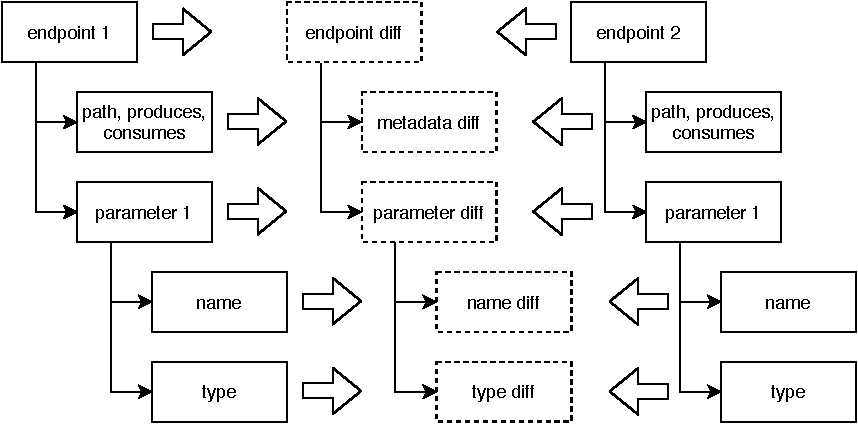
\includegraphics{diff-construction}
%	\caption{Vytvoření diffů}
%	\label{fig:diff-construction}
%\end{figure}

\section{Algoritmus porovnání}

Porovnávací algoritmus pracuje s metadaty popsanými v části \ref{subsec:crce-metadata}. Jedná se o stromovou strukturou, jejíž uzly tvoří instance tříd \textit{Capability}, \textit{Property} a \textit{Attribute}, kde objekty \textit{Attributes} jsou listy této struktury . Soubor metadat může obsahovat další vlastnosti komponenty, která představuje webovou službu, ta však zůstanou nedotčena, protože algoritmus pracuje pouze s daty, která byla vytvořena indexery popsanými v části \ref{sec:api-index}.

Moduly pro indexování webových služeb popsané v předchozí kapitole používají dvě různé množiny \textit{namespace} identifikátorů po pojmenování entit (\textit{Capability}, \textit{Property}, \textit{Attribute}). Do budoucna je zároveň plánované rozšíření těchto modulů o funkcionalitu pro indexování datových typů a datová struktura metadat je tedy předmětem změny. Z těchto důvodů je algoritmus schopen porovnat pouze metadata z jednoho indexeru. Není tedy možné vzájemně porovnat například metadata REST služby získaná binární analýzou JAR s metadaty získanými čtením JSON-WSP dokumentu i když by se mohlo jednat o jednu službu.

%- zmínit taky omezení, která plynou z indexovaných dat

\subsection{Složitost algoritmu}

\begin{itemize}
	\item REST služby: $O(n^2)$ kde $n$ je počet endpointů
	\item WADL, JSON-WSP: $O(n^2)$ kde $n$ je počet endpointů
	\item WSDL: $O(m\cdot n^2)$ kde $m$ je počet WS a $n$ je počet endpointů ve WS
\end{itemize}

\subsection{Popis algoritmu}

Vstup algoritmu: reprezentace obou webových služeb v podobě \textit{Resource}. Výstupem algoritmu: objekt \textit{Compatibility}.

Před porovnáváním datových struktur je zkontrolována jejich kompatibilita: typ popisu, \textit{communication pattern}, \textit{identity capability}. Pokud kontrola proběhne úspěšně, je spuštěn samotný algoritmus jehož průběh je naznačen na vývojovém diagramu \ref{fig:apicomp-flow}. V případě porovnání SOAP webových služeb je tento postup obalen ještě porovnáním \textit{services}, které WSDL definuje a které jsou v CRCE reprezentovány jako kolekce endpointů.

\begin{figure}[h]
	\centering
	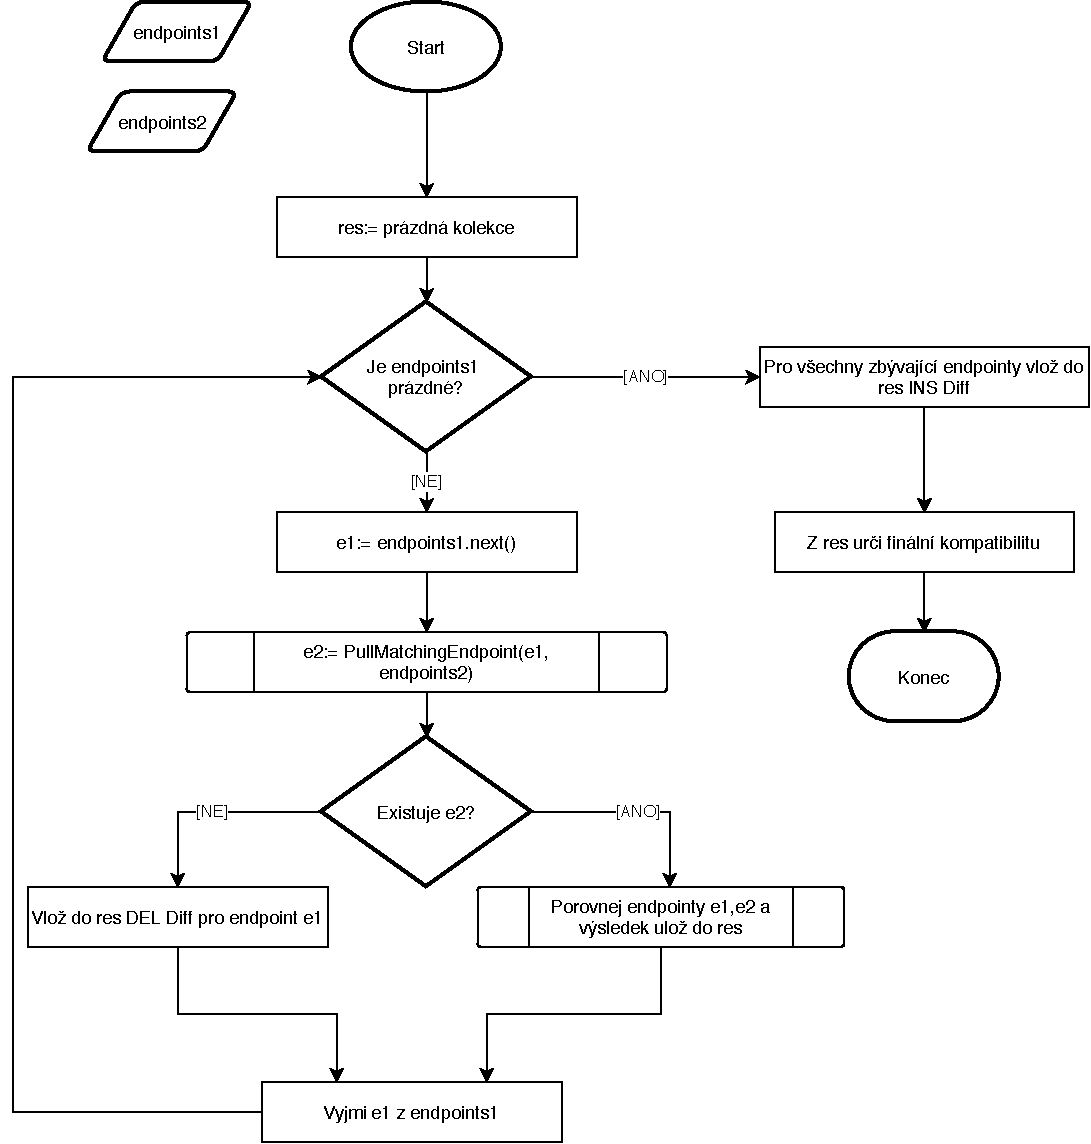
\includegraphics[width=10cm]{apicomp-flow}
	\caption{Vývojový diagram porovnávacího algoritmu}
	\label{fig:apicomp-flow}
\end{figure}

Mezivýsledky porovnání jsou ukládány v datové struktuře \textit{Diff}, která je detailně popsaná v sekci \ref{sec:diff-info}. Algoritmus postupuje po stromu metadat od kořene směrem k listům. V listech dojde k porovnání konkrétních hodnot. Pokud jsou porovnány všechny potomci uzlu, je vyhodnocena jeho kompatibilita. Takto se postupuje zpět ke kořeni stromu, který na konci algoritmu obsahuje finální údaj o kompatibilitě dvou API. Jednotlivé fáze porovnání jsou popsány v následujících odstavcích.

\paragraph{Výběr endpointu vhodného k porovnání}

Protože nelze předpokládat pořadí endpointů v metadatech, je nutné před samotným porovnáním nejprve vybrat dvojici endpointů k tomu vhodnou. Endpoint z první webové služby (\textit{e1}) je vybrán sekvenčně (jak je naznačeno na \ref{fig:apicomp-flow}). Druhý endpoint (\textit{e2}) je pak vybrán na základě určité shody s metadaty endpointu \textit{e1}, konkrétně se jedná o počet povinných parametrů, jméno a URL na které jsou endpointy dostupné. URL nemusí být shodné úplně, pokud tak nastane, je nastavena vlajka MOV, která je detailně popsána v sekci \ref{subsec:mov}.

O porovnatelnosti dvou \textit{services} (v případě SOAP) je rozhodnuto na základě úplné shody jejich jmen.

\paragraph{Porovnání dvou services}
Asi jen název.

\paragraph{Porovnání dvou endpointů}
Po výběru vhodné dvojice endpointů dojde k jejich porovnání. Postupně se porovnají (pokud jsou pro daný typ webové služby definovány) parametry, response a request. 

\paragraph{Porovnání parametrů endpointů}
Je porovnáváno: jméno, pořadí, datový typ, případně povinnost. V případě GEN/SPE u datového typu parametru je použita kontravariance a výsledná hodnota je opačná.

\subsection{Porovnání datových typů}
V současnosti jsou největším omezením porovnávacího algoritmu datové typy. Jako již bylo zmíněno v kapitole \ref{sec:api-index}, jméno datového typu je jedinou dostupnou informací a tedy také jediným kritériem, podle kterého je lze porovnávat. To je dostatečné v případě vestavěných typů jako například třídy z balíku \verb|java.lang|, nebo typy definované v xsd. 

Nad těmito lze provádět plnohodnotné porovnání včetně kontroly generalizace. U vestavěných typů Javy je generalizace určena na základě dědičnosti a lze například určit, že typ s názvem \verb|java.lang.Number| je generalizací typu s názvem \verb|java.lang.Long|, protože třída \textit{Number} je rodičem třídy \textit{Long}. Obdobně je tomu i u vestavěných typů definovaných v xsd, kde je generalizace $a <: b$ definována v případě, že typ $b$ je dost velký na pojmutí typu $a$. Například typ \verb|xsd:long| dokáže reprezentovat číslo typu \verb|xsd:int| a proto platí, že $xsd:int <: xsd:long$. 

Porovnání vestavěných typů je založeno na podmínce správně zaindexovaného jména datového typu. V případě analýzy byte kódu je tato podmínka splněna, nicméně u metadat získaných čtením popisných XML souborů tomu tak vždy nemusí být. Problém spočívá v  předponě datového typu, která je součástí jeho jména a porovnávací algoritmus očekává její určitou hodnotu (konkrétně \verb|xs|). Hodnota předpony je však určena definicí namespace v XML popisu a ta se může od očekávané lišit. Tato definice není indexerem ukládána a není proto možné ji během porovnání přesně určit.

Pro uživatelsky definované typy je porovnání omezeno pouze na úplnou shodu, protože na základě pouhého jména datového typu nejde s jistotou usoudit nic dalšího.
	
\section{MOV flag}	
\label{subsec:mov}
Popis MOV

Co: Příznak označující, že API/endpoint má (částečně) shodnou implementaci, ale nachází se na jiné adrese

Proč: endpointy v API mohou mít jiné url/jména, ale implementačně mohou být shodné -> potřeba detekovat

Jak: na základě ostatních metadat (počet parametrů, počet endpointů ve WS)

Mov se také nastaví pokud je zaplé ignorování verzi REST API v endpoint path a pokud: 
\begin{itemize}
	\item cesty s verzí nejsou stejné
	\item cesty bez verze jsou stejné
\end{itemize}

Algorimuts (nemusí vždy fungovat správně):
\begin{itemize}
	\item  obecná detekce před samotným porovnáním -> MovDetectionResult
	\item  3x diff: host, path to endpoint, operace
	\item  MovDetectionResult se pak použije při výběru endpointu k porovnání a při samotném porovnání (pickBest)
\end{itemize}
	
- kombinace které vedou na mov: 
\begin{itemize}
	\item $h \land !pe \land !o$
	\item $h \land pe \land !o$
	\item TODO
\end{itemize}

\subsection{Verze REST API v cestě k endpointu}	
\label{sec:api-path-version}

Proč: 

\begin{itemize}
	\item klient může chtít volat novou verzi API a je tedy žádané zjistit, jak moc je API kompatibilní (např. se mohla změnit jen implementace, takže signatura je stále stejná)
	
	\item Normálně by algoritmus skončil MUT, protože by kvůli rozdílným cestám k endpointům vyhodnotil endpointy z API 1 jako DEL a endpointy z API 2 jako INS
	
	\item to není žádané, takže algoritmus je schopný detekovat verzi v cestě k endpointu a při výběru endpointů k porovnání ji ignorovat
\end{itemize}

Podporovaný formát:
\begin{itemize}
	\item \verb|v<major>[.minor[.micro]]|
	\item lowecase i uppercase
	\item oddělovač může být '.', nebo '-'
	\item regex: \verb|\/[vV][0-9]+(?:[.-][0-9]+){0,2}\/|
\end{itemize}

Detekci verze je možno vypnout. Pokud je detekce zapnutá, algoritmus se před porovnáním cest pokusí najít verzi a pokud ji najde, z cesty ji vyřadí a porovná cesty bez verze

\section{Vyhodnocení výsledků}

- jak probíhá vyhodnocení (nejdříve se určí hodnoty listů, z nich se pak počítá dál nahoru)

- kontravariance

	- není to úplně problém, ale při vyhodnocování finálního Diffu pro endpoint je potřeba brát v potaz 
	
	- GEN/SPE může vzniknout jen z datových typů parametrů/response endpointu, takže je to poměrně přímočaré

\begin{table}[h!]
	\centering
	\begin{tabular}{|l|c|}
		\hline
		Difference & Dopad na klienta  \\
		\hline
		\hline
		None (NON) & bezpečné \\
		\hline
		Specialization (SPE) & bezpečné  \\
		\hline
		Insertion (INS) & bezpečné \\
		\hline
		Deletion (DEL) & potenciálně nebezpečné \\
		\hline
		Generalization (GEN) & potenciálně nebezpečné \\
		\hline
		Mutation (MUT) & nebezpečné \\
		\hline
		Unkown (UNK) & nebezpečné \\
		\hline
	\end{tabular}
	\caption{Dopad jednotlivých úrovní rozdílu na klienta }
	\label{tab:diff-level}
\end{table}

\chapter{Implementační detaily (jen stručně)}

 - zmínit, proč třídy pro porovnávání REST API a WS nemají společného předka (krom rozhraní)
 	- důvod: chtěl jsem nechat implementaci obou porovnávačů oddělenou pro případ, že by se změnila funkce indexerů

\chapter{Testování}

- nějaká reálná data
	- STAG (WSDL)
	- Fuel Economy
- i syntetická data
- algoritmus testován pomocí unit testů

\section{Integrační + akceptační testy}

- testování skrze REST API
- pomocí Postman (Collection Runner)
- několik verzí jednoho API -> testování křížem
- todo: příklad
	- popsat verze API (čím se liší), případně zdůvodnit očekávaný výsledek
	- tabulka vzájemného porovnání s výsledky

\subsection{Syntetický server v Jave}
\begin{itemize}
	\item postaveno na Jersey
	\item REST API
	\item alespoň obrázek/raml api?
	\item 2 verze otestované křížem
\end{itemize}

Popis verzí API (rozdíl je vždy popsaný oproti verzi 1):
\begin{itemize}
	\item V1: základní verze
	\item V2: typ parametru změněn z Long na Number
\end{itemize}

Co se testuje:
\begin{itemize}
	\item GEN/SPEC a kontravariance u parametru endpointu
\end{itemize}	
	
\subsection{Příklad JSON-WSP z wiki}

\begin{itemize}
	\item popsáno JSON-WSP souborem
	\item https://en.wikipedia.org/wiki/JSON-WSP
	\item 4 verze otestované křížem
\end{itemize}

Popis verzí API (rozdíl je vždy popsaný oproti verzi 1):
\begin{itemize}
	\item V1: základní verze
	\item V2: typ User je jiný
	\item V3: přidána metoda deleteUser
	\item v4: metoda listGroups změněna na getUsersInGroup
\end{itemize}

Co se testuje:
\begin{itemize}
	\item ne-indexování custom datových typů (takže v2 = v1)
	\item mutace endpointu
	\item INS, DEL
\end{itemize}

\subsection{FuelEconomy API}

\begin{itemize}
 \item popsáno WADL souborem
 \item https://www.fueleconomy.gov/ws/rest/application.wadl
 \item 3 verze otestované křížem
\end{itemize}

Popis verzí API (rozdíl je vždy popsaný oproti verzi 1):
\begin{itemize}
	\item V1: základní verze
	\item V2: odebrán (poslední) resource /labelvehicle
	\item V3: odebrán (poslední) resource /labelvehicle, přidán resource /somethingDifferent
\end{itemize}

Co se testuje:
\begin{itemize}
	\item  INS, DEL a MUT
\end{itemize}

\subsection{Stag WS}

TODO

\chapter{Závěr}	

 
% 
% PRO ANGLICKOU SAZBU JE NUTNÉ ZMĚNIT
% CITAČNÍ STYL!
%
\bibliographystyle{csplainnatkiv}
{\raggedright\small
\bibliography{literatura}
}

% seznam zkratek
\chapter*{Seznam zkratek}
\addcontentsline{toc}{chapter}{Seznam zkratek}

\begin{longtable}{@{}p{3cm}@{}p{\dimexpr\textwidth-1cm\relax}@{}}
	\nomenclature{CRCE}{Component Repository supporting Compatibility Evaluation}
	\nomenclature{API}{Application Programming Interface}
	\nomenclature{HTTP}{Hypertext Transfer Protocol}
	\nomenclature{JAR}{Java Archive}
	\nomenclature{JSON}{JavaScript Object Notation}
	\nomenclature{JSON}{JSON Web-Service Protocol}
	\nomenclature{OSGi}{Open Services Gateway initiative}
	\nomenclature{REST}{Representational State Transfer}
	\nomenclature{SOAP}{Simple Object Access Protocol}
	\nomenclature{UML}{Unified Modeling Language}
	\nomenclature{URI}{Uniform Resource Identifier}
	\nomenclature{URL}{Uniform Resource Locator}
	\nomenclature{WADL}{Web Application Description Language}
	\nomenclature{WSDL}{Web Services Description Language}
	\nomenclature{XML}{Extensible Markup Language}
	\nomenclature{XSD}{XML Schema Definition}
\end{longtable}

\end{document}
